%!TEX root = parita-msc.tex

\chapter{Proof of Concept}\label{chap:proofOfConcept}

\begin{doublespace}

Chapter~\ref{chap:methodology} focuses on the methodology which has been followed to describe and publish the linked open vocabulary for survey in this chapter.

\section{OWL Ontology for Survey Using Protégé}

Figure~\ref{feedback-form} shows the student feedback form for which the new vocabularies are described. 

\begin{figure}[htp]
    \centering
    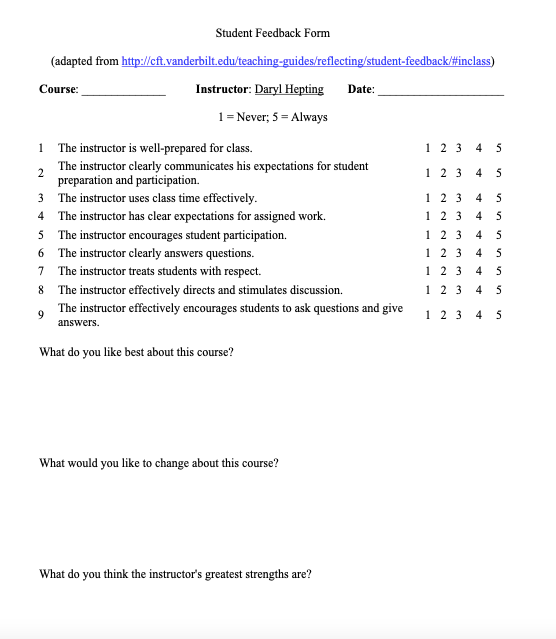
\includegraphics[width=15cm]{images/ch4/survey/feedback-form.png}
    \caption{The Student Feedback Form, from Hepting~\cite{prof}}
    \label{feedback-form}
\end{figure}

\subsection{Classes for Survey Ontology}

All the classes can be created and described using the steps described in section~\ref{subsec:classhierarchy}. The resultant class hierarchy for the survey ontology would be as shown in Figure~\ref{survey-class-hierarchy}. A survey can have \say{Survey Response}, \say{Respondent}, \say{Response Date}, \say{Type of Survey}, \say{Survey Questions}, and \say{Survey Answers}, which are considered for this ontology as well. 

\begin{figure}[htp]
    \centering
    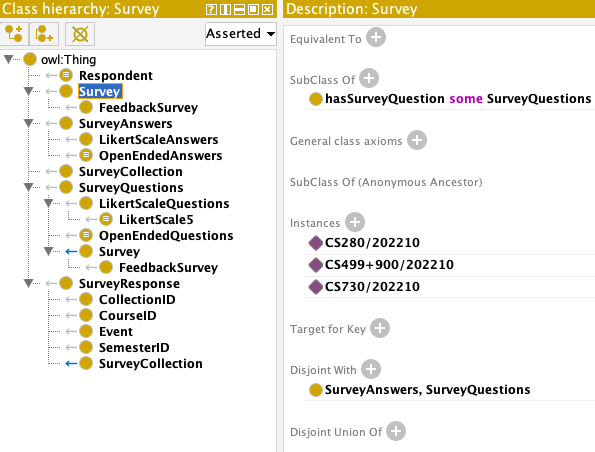
\includegraphics[width=15cm]{images/ch4/survey/survey-class-hierarchy.png}
    \caption{Class Hierarchy in Survey Ontology}
    \label{survey-class-hierarchy}
\end{figure}

Here, the type of survey used is feedback survey (\say{FeedbackSurvey} class). The \say{SurveyCollection} class corresponds to a collection of survey responses (\say{SurveyResponse} class) that were collected for a particular course (\say{CourseID} class) in a particular semester (\say{SemesterID} class) with a specific collection ID (\say{CollectionID} class). Furthermore, the survey questions and survey answers have classes corresponding to various forms of question-answer. Generally, feedback surveys consist of two types of questions, namely, \say{Likert Questions} and \say{Open-ended Questions}. The type of questions might differ depending on the designer of the survey, some of which, as stated on the \emph{SurveyMonkey}\footnote{https://www.surveymonkey.com/mp/survey-question-types/} website, are listed below. 

\begin{multicols}{2}
\begin{itemize}
   
    \item Multiple Choice Questions
   
    \item Rating Scale Questions
   
    \item Likert Scale Questions
   
    \item Matrix Questions
   
    \item Dropdown Questions
   
    \item Open-ended Questions
   
    \item Demographic Questions
   
    \item Ranking Questions
   
    \item Image Choice Questions
   
    \item Click Map Questions
   
    \item File Upload Questions
   
    \item Slider Questions
   
    \item Benchmarkable Questions

\end{itemize}
\end{multicols}

The feedback survey in this research has Likert and Open-ended questions. The classes described for the questions and answers are \say{LikertScaleQuestions}, and \say{OpenEndedQuestions} as sub-classes of \say{SurveyQuestions}, and \say{LikertScaleAnswers}, and \say{OpenEndedAnswers} as sub-classes of \say{SurveyAnswers}. For all the survey questions, there is a question and an answer, where both of them are considered as distinct classes. Open-ended questions have unpredictable answers.

\subsubsection{The ``LikertScaleQuestions'' Class}

Likert questions are the questions for which the answers are from the preset list of answers. For the Likert questions, the questions can be either of type \say{Never-Always-4} or \say{Never-Always-5} or \say{Never-Always-7} or \say{Never-Always-*}, of which Never-Always-5 has been used by Hepting~\cite{prof}. The survey ontology consists of \say{LikertScaleQuestions} class for likert questions.

In a Never-Always-5 type of survey, 5 degrees of agreement can be used. It is challenging to decide whether the range for the degrees would be 0 to 4, 1 to 5, 10 to 50, or something else. The degree of agreements used here are as shown in Table~\ref{likert-degrees}. In addition to these degrees, this ontology also considers the instances where the question wouldn't be answered. In this case, the field corresponding to the answer is left blank.

\begin{table}[h!]
    \centering
    \begin{tabular}{|c|l|}
    \hline Number \ & Agreement \\ \hline
     1 & Never\\ \hline
     2 & [Rarely]\\ \hline
     3 & [Sometimes]\\ \hline
     4 & [Often]\\ \hline
     5 & Always\\ \hline
    \end{tabular}
    \caption{Degrees of Agreement for Likert-scale Questions}
    \label{likert-degrees}
\end{table}

The \say{LikertScaleQuestions} class of survey ontology has a sub-class, \say{LikertScale5}, which represents the likert scale with the degrees of agreement from Table~\ref{likert-degrees}. The \say{Equivalent To} (from the description view of the class tab) can be used to describe the \say{LikertScale5} class in terms of a range containing degrees of agreement as shown in Figure~\ref{likertscale5-class}. Each of these degrees are treated as an individual (section~\ref{subsec:individuals}) of the class.

\begin{figure}[htp]
    \centering
    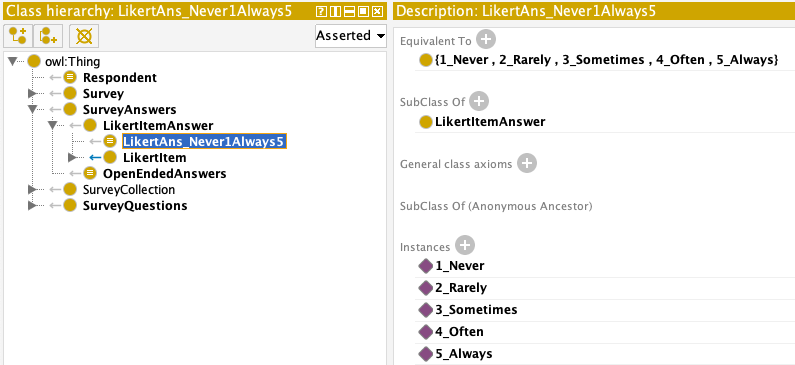
\includegraphics[width=15cm]{images/ch4/survey/likertscale5-class.png}
    \caption{``LikertScale5'' class in Survey Ontology}
    \label{likertscale5-class}
\end{figure}

\subsection{Object Properties for Survey Ontology}

Using the method of naming and building object properties described in section~\ref{subsec:objectproperties}, some of the primary object properties are described for the survey ontology as shown in Figure~\ref{survey-object-properties} where as Table~\ref{survey-object-properties-domains-and-ranges} shows the list of the object properties along with their domain and range classes. Table~\ref{survey-object-properties-parent-nodes-and-inverse} consists of the parent nodes and inverse properties of the object properties. The three parent nodes involved in object property hierarchy are \say{owl:TopObjectProperty}, \say{hasContent}, and \say{isContentOf}.

\begin{figure}[htp]
    \centering
    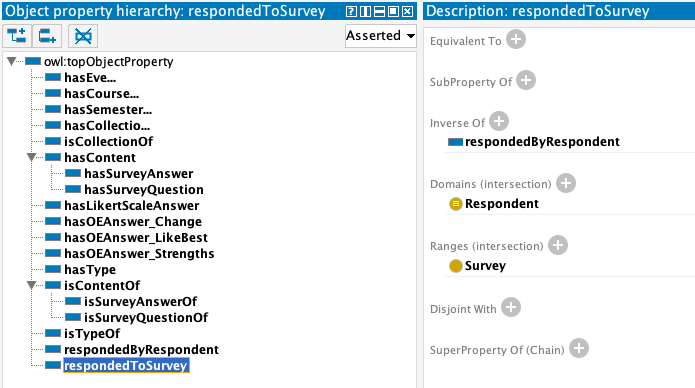
\includegraphics[width=15cm]{images/ch4/survey/survey-object-properties.png}
    \caption{Object Property Hierarchies, Domain and Range for Classes}
    \label{survey-object-properties}
\end{figure}

\begin{table}[h!]
    \centering
    \begin{tabular}{|l|l|l|} 
    \hline \ \ \ \ \ Object Property & \ \ \ \ \ \ \ \ Domain & \ \ \ \ \ \ \ \ Range\\ \hline
     hasSurveyQuestion & Survey & SurveyQuestions\\ \hline
     hasSurveyAnswer & Survey & SurveyAnswers\\ \hline
     hasOEAnswer\_Change & OpenEndedQuestions & OpenEndedAnswers\\ \hline
     hasOEAnswer\_LikeBest & OpenEndedQuestions & OpenEndedAnswers\\ \hline
     hasOEAnswer\_Strengths & OpenEndedQuestions & OpenEndedAnswers\\ \hline
     hasLikertScaleAnswer & LikertScaleQuestions & LikertScale5\\ \hline
     hasEvent & SurveyResponse & Event\\ \hline
     hasCourseID & SurveyResponse & CourseID\\ \hline
     hasSemesterID & SurveyResponse & SemesterID\\ \hline
     hasCollectionID & SurveyResponse & CollectionID\\ \hline
     isCollectionOf & SurveyCollection & SurveyResponse\\ \hline
     respondedToSurvey & Respondent & Survey\\ \hline
     isTypeOf & FeedbackSurvey & Survey\\ \hline
    \end{tabular}
    \caption{Object Properties and Their Domain and Range}
    \label{survey-object-properties-domains-and-ranges}
\end{table}

\begin{table}[h!]
    \centering
    \begin{tabular}{|l|l|l|} 
    \hline \ \ \ \ \ Object Property & \ \ \ \ \ \ \ Parent Node & \ \ \ \ \ Inverse Property\\ \hline
     hasContent & owl:TopObjectProperty & isContentOf\\ \hline
     isContentOf & owl:TopObjectProperty & hasContent\\ \hline
     hasType & owl:TopObjectProperty & isTypeOf\\ \hline
     isTypeOf & owl:TopObjectProperty & hasType\\ \hline
     hasLikertScaleAnswer & owl:TopObjectProperty & \\ \hline
     hasOEAnswer\_Change & owl:TopObjectProperty & \\ \hline
     hasOEAnswer\_LikeBest & owl:TopObjectProperty & \\ \hline
     hasOEAnswer\_Strengths & owl:TopObjectProperty & \\ \hline
     hasEvent & owl:TopObjectProperty & \\ \hline
     hasCourseID & owl:TopObjectProperty & \\ \hline
     hasSemesterID & owl:TopObjectProperty & \\ \hline
     hasCollectionID & owl:TopObjectProperty & \\ \hline
     isCollectionOf & owl:TopObjectProperty & \\ \hline
     respondedByRespondent & owl:TopObjectProperty & respondedToSurvey\\ \hline
     respondedToSurvey & owl:TopObjectProperty & respondedByRespondent\\ \hline
     hasSurveyQuestion & hasContent & isSurveyQuestionOf\\ \hline
     hasSurveyAnswer & hasContent & isSurveyAnswerOf\\ \hline
     isSurveyQuestionOf & isContentOf & hasSurveyQuestion\\ \hline
     isSurveyAnswerOf & isContentOf & hasSurveyAnswer\\ \hline
    \end{tabular}
    \caption{Object Properties with Their Parent Nodes and Inverse Properties}
    \label{survey-object-properties-parent-nodes-and-inverse}
\end{table}

\subsection{Data Properties for Survey Ontology}

Data properties for survey ontology have been described following the method described in section~\ref{subsec:dataproperties} which are as shown in Figure~\ref{survey-data-properties}.

\begin{figure}[htp]
    \centering
    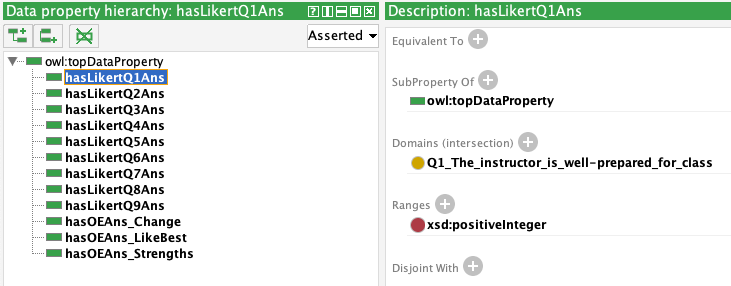
\includegraphics[width=15cm]{images/ch4/survey/survey-data-properties.png}
    \caption{Data Property Hierarchies, Domain and Range for Classes}
    \label{survey-data-properties}
\end{figure}

The parent node of all the data properties is \say{owl:topDataProperty} and the domain and range for all the data properties are listed in Table~\ref{survey-data-properties-domains-and-ranges}. The properties for likert answers restrict the datatype to positive integer and to string for open-ended answers.

\begin{table}[h!]
    \centering
    \begin{tabular}{|l|l|l|} 
    \hline \ \ \ \ \ \ \ \ \ \ \ \ \ \ \ Data Property &\ \ \ Domain &\ \ \ \ \ \ \ Range\\ \hline
     hasLikertAns\_is\_well-prepared\_for\_class & Respondent & xsd:positiveInteger\\ \hline
     hasLikertAns\_clearly\_communicates\_his\_expecta-&\\ tions\_for\_student\_preparation\_and\_participation & \multirow{-2}{5em}{Respondent} & \multirow{-2}{8.5em}{xsd:positiveInteger}\\ \hline
     hasLikertAns\_uses\_class\_time\_effectively & Respondent & xsd:positiveInteger\\ \hline
     hasLikertAns\_has\_clear\_expectations\_for&\\ \_assigned\_work & \multirow{-2}{5em}{Respondent} & \multirow{-2}{8.5em}{xsd:positiveInteger}\\ \hline
     hasLikertAns\_encourages\_student\_participation & Respondent & xsd:positiveInteger\\ \hline
     hasLikertAns\_clearly\_answers\_questions & Respondent & xsd:positiveInteger\\ \hline
     hasLikertAns\_treats\_students\_with\_respect & Respondent & xsd:positiveInteger\\ \hline
     hasLikertAns\_effectively\_directs\_and\_stimulates&\\ \_discussion & \multirow{-2}{5em}{Respondent} & \multirow{-2}{8.5em}{xsd:positiveInteger}\\ \hline
     hasLikertAns\_effectively\_encourages\_students\_to&\\ \_ask\_questions\_and\_give\_answers & \multirow{-2}{5em}{Respondent} & \multirow{-2}{8.5em}{xsd:positiveInteger}\\ \hline
     hasOEAnswer\_Change & Respondent & xsd:string\\ \hline
     hasOEAnswer\_LikeBest & Respondent & xsd:string\\ \hline
     hasOEAnswer\_Strengths & Respondent & xsd:string\\ \hline
    \end{tabular}
    \caption{Data Properties and Their Domain and Range}
    \label{survey-data-properties-domains-and-ranges}
\end{table}

\subsection{Individuals}\label{subsec:individuals}

While dealing with ontologies, an instance of class is termed as an \say{Individual}. In protégé, an individual can be described as an instance of class using the Description view of the Class tab. For example, Figure~\ref{instances-of-survey-class} shows instances of \say{Survey} class.

\begin{figure}[htp]
    \centering
    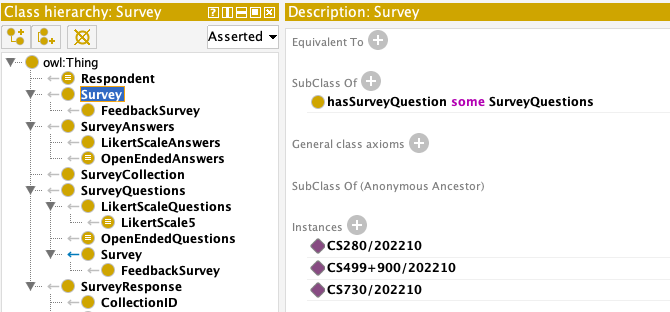
\includegraphics[width=15cm]{images/ch4/survey/instances-of-survey-class.png}
    \caption{Individuals for Survey Class}
    \label{instances-of-survey-class}
\end{figure}

A new individual can be described using the Individuals view of the Entities tab where as the property assertions view can be used to describe the property restrictions. Table~\ref{survey-individuals} shows a list of classes and individuals described in survey ontology.

\begin{table}[h!]
    \centering
    \begin{tabular}{|l|l|} 
    \hline \ \ \ \ \ \ \ \ \ \ Class & \ \ \ \ \ \ \ \ \ \ \ \ \ \ \ \ \ \ \ \ \ \ \ \ \ \ \ \ \ Individuals \\ \hline
     Respondent &  1, 2, 3, ... , 59 \\ \hline
     Survey & CS280/202210, CS499+900/202210, CS730/202210 \\ \hline
     SurveyCollection &  Collection1, Collection2 \\ \hline
     Event &  FinalExam, Midterm \\ \hline
     CollectionID &  CS280/202210/Collection1 \\ \hline
     SemesterID &  202210, 202220, 202230 \\ \hline
     CourseID &  CS280, CS499+900, CS730 \\ \hline
     \multirow{2}{9.5em}{OpenEndedQuestions} &  OEQuestion\_LikeBest, OEQuestion\_Change, \\& OEQuestion\_Strengths \\ \hline
     OpenEndedAnswers & OEAns\_LikeBest, OEAns\_Change, OEAns\_Strengths \\ \hline
     LikertScale5 & 1\_Never, 2\_Rarely, 3\_Sometimes, 4\_Often, 5\_Always \\ \hline
    \end{tabular}
    \caption{Classes and their Individuals}
    \label{survey-individuals}
\end{table}

\subsection{Final Class Hierarchy for Survey Ontology}

The final class hierarchy of the \ac{owl} ontology in protégé, after using the HermiT 1.4.3.456 reasoner, would be as shown in Figure~\ref{final-survey-classes}.

\begin{figure}[htp]
    \centering
    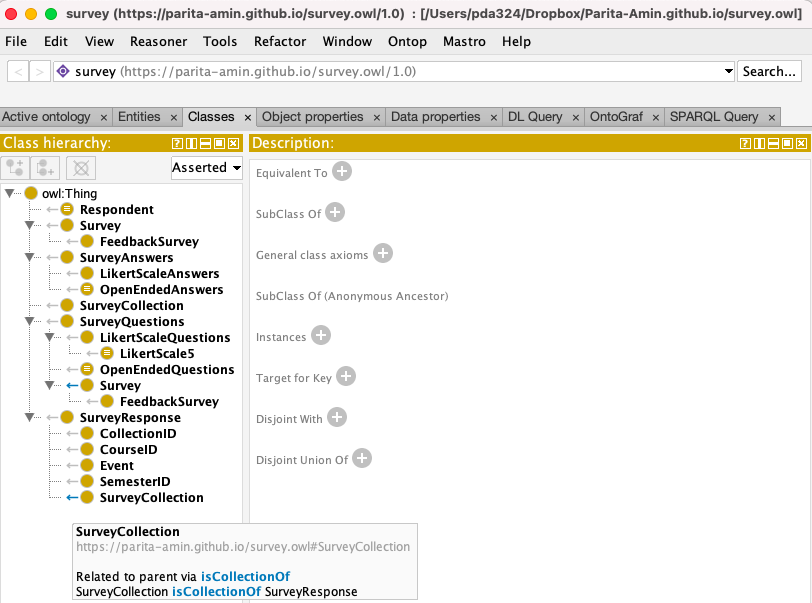
\includegraphics[width=15cm]{images/ch4/survey/final-survey-classes.png}
    \caption{Class Hierarchy for the Final Version of Survey Ontology}
    \label{final-survey-classes}
\end{figure}

The blue (\say{Survey} and \say{SurveyCollection} class) back arrow in front of the yellow solid dot, which indicates class, show parent/child relationship other than that of SubClassOf. This feature can be enabled and disabled by selecting \say{Display relationship in class hierarchy} option from the \say{View} menu of protégé. Figure~\ref{final-survey-classes} shows the relation indicated by the blue back arrow.

\subsection{Using SHACL for Data Validation}

\ac{shacl}4P is a protégé plugin for \ac{shacl}, which uses \say{shapes} to describe constraints. \ac{shacl} can be used to validate the manually entered data which are stored in spreadsheets. For feedback survey, the likert answers can only have values 1, 2, 3, 4, 5, or No Answer (blank cell). To restrict the values of data properties corresponding to likert questions in Figure~\ref{survey-data-properties}, \ac{shacl}4P has been used.

Protégé offers a view for \ac{shacl} editor as well as \ac{shacl} constraint violations. For successful working of \ac{shacl}4P, a reasoner should be enabled. The \ac{shacl} editor provides three buttons, namely, \say{Open}, \say{Save} , and \say{Validate}. After opening the shapes file (Open button), changes can be made and saved (Save button). Where as the Validate button allows users to validate the data. Figure~\ref{shacl-editor} shows a sample \say{SurveyShapes.txt} file opened in \ac{shacl} editor of protégé.

\begin{figure}[htp]
    \centering
    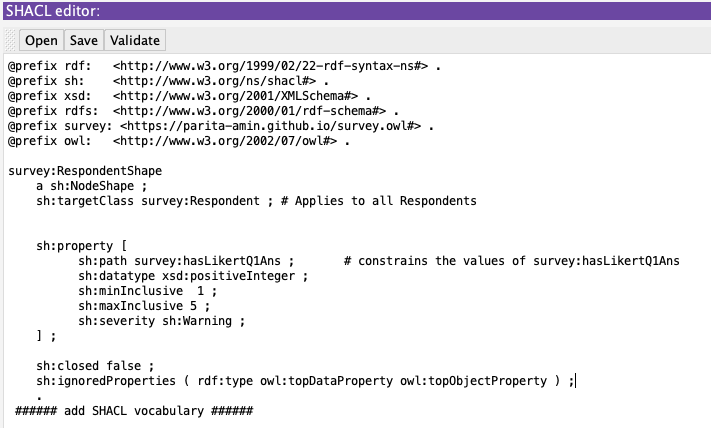
\includegraphics[width=15cm]{images/ch4/survey/shacl-editor.png}
    \caption{Data Validation using SHACL Editor}
    \label{shacl-editor}
\end{figure}

On clicking the Validate button, the summary of violated constraints is displayed on the \ac{shacl} constraint violations view in protégé. It contains the details like \say{Severity}, \say{SourceShape}, \say{Message}, \say{FocusNode}, \say{Path}, and \say{Value} as shown in Figure~\ref{shacl-constraint-violations}.

\begin{figure}[htp]
    \centering
    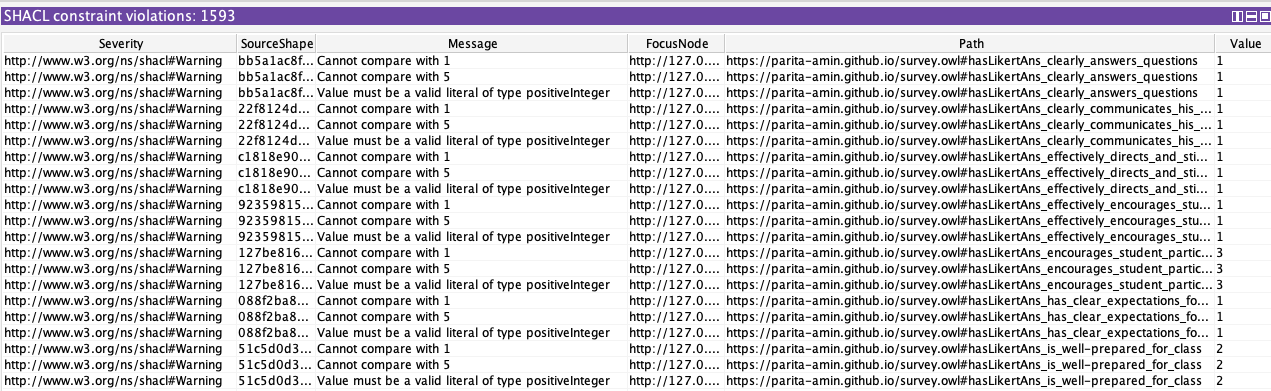
\includegraphics[width=15cm]{images/ch4/survey/shacl-constraint-violations.png}
    \caption{SHACL Constraint Violations}
    \label{shacl-constraint-violations}
\end{figure}

\subsection{Querying Survey Ontology in Protégé}

The ontology vocabularies can be queried using query languages like DL query and \ac{sparql}. A DL query is used to  such as `and' (corresponding to set intersection) and `some'.\footnote{https://ontology101tutorial.readthedocs.io/en/latest/EXERCISE\_BasicDL\_Queries.html}. \ac{sparql} query is used to express queries and optional graph patterns along with their conjunctions and disjunctions as well as aggregation, subqueries, negation, etc.\footnote{https://www.w3.org/TR/sparql11-query/} 

Protégé offers a plugin for DL as well as SPARQL queries. 

\subsubsection{DL Query}

\say{The DL Query tab allows users to quickly test definitions of classes to see that they subsume the appropriate subclasses. Or check for class membership of arbitrary descriptions without having to create named class placeholders.}\footnote{https://protegewiki.stanford.edu/wiki/DL\_Query} The DL Query tab can be opened using Tabs option under Windows menu. It is important to configure a reasoner to successfully express a DL query. Figure~\ref{survey-dl-query} shows expression of a sample DL query on the survey ontology in protégé. 

\begin{figure}[htp]
    \centering
    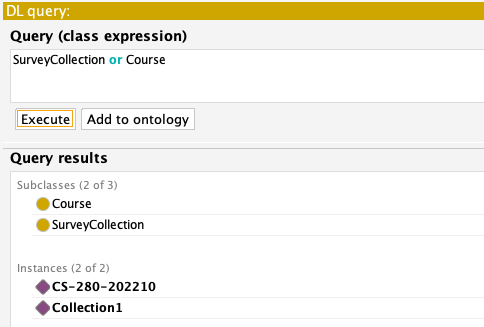
\includegraphics[width=15cm]{images/ch4/survey/survey-dl-query.png}
    \caption{DL Query on Survey Ontology}
    \label{survey-dl-query}
\end{figure}

\subsubsection{SPARQL Query}



\begin{figure}[htp]
    \centering
    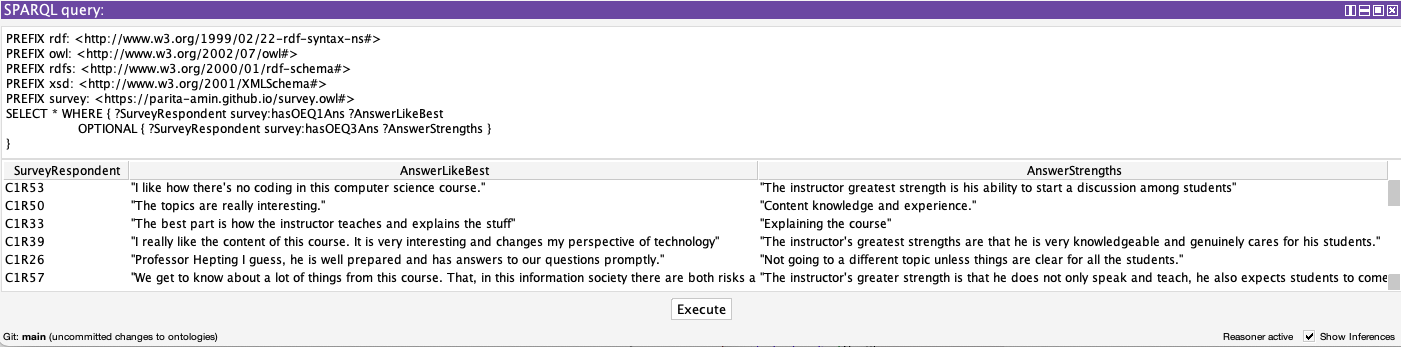
\includegraphics[width=15cm]{images/ch4/survey/survey-sparql-query.png}
    \caption{SPARQL Query on Survey Ontology}
    \label{survey-sparql-query}
\end{figure}

\begin{figure}[htp]
    \centering
    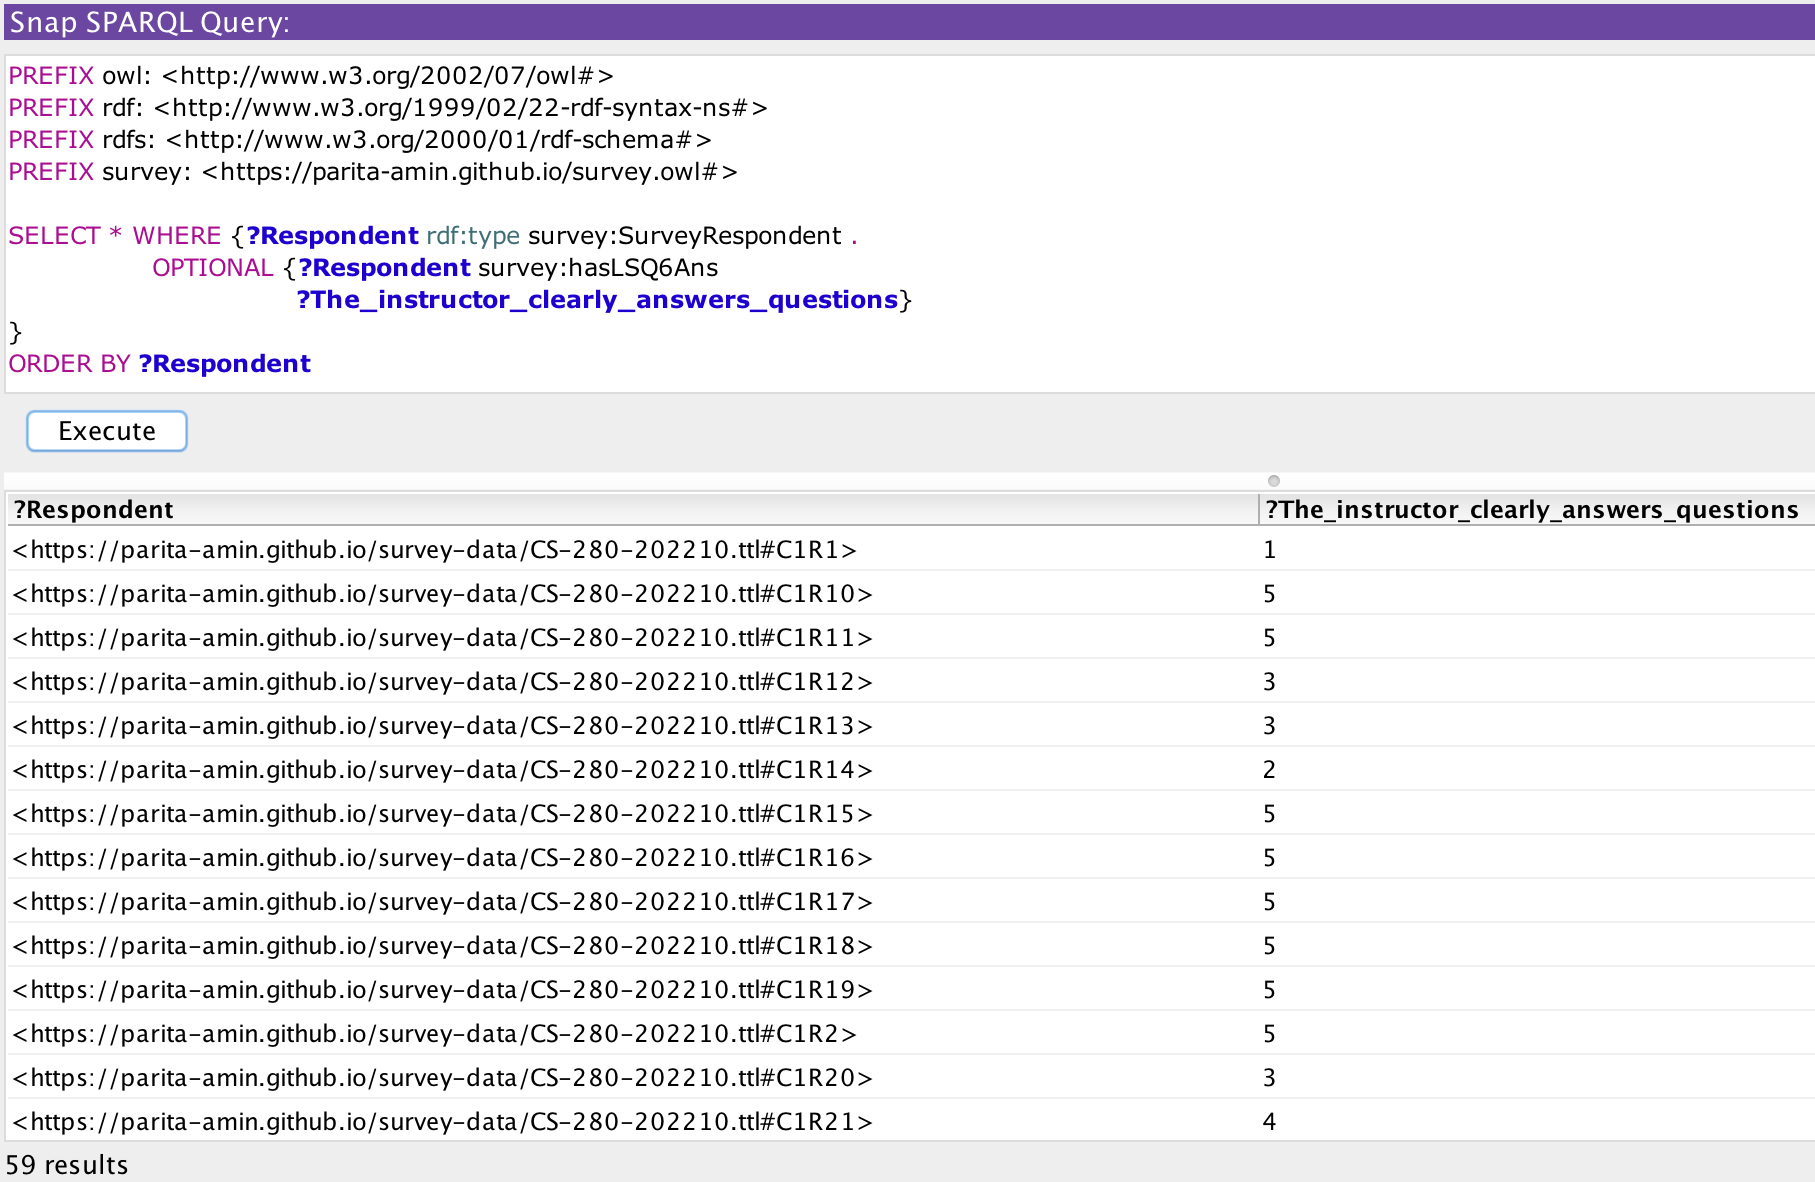
\includegraphics[width=15cm]{images/ch4/survey/survey-snap-sparql-query.png}
    \caption{Snap SPARQL Query on Survey Ontology}
    \label{survey-snap-sparql-query}
\end{figure}

\section{From Spreadsheets to Linked Open Data For Survey Ontology}

Primarily, OpenRefine\footnote{https://openrefine.org/} was used to convert the data stored in spreadsheets to Turtle and \ac{rdf} files.

\begin{figure}[htp]
    \centering
    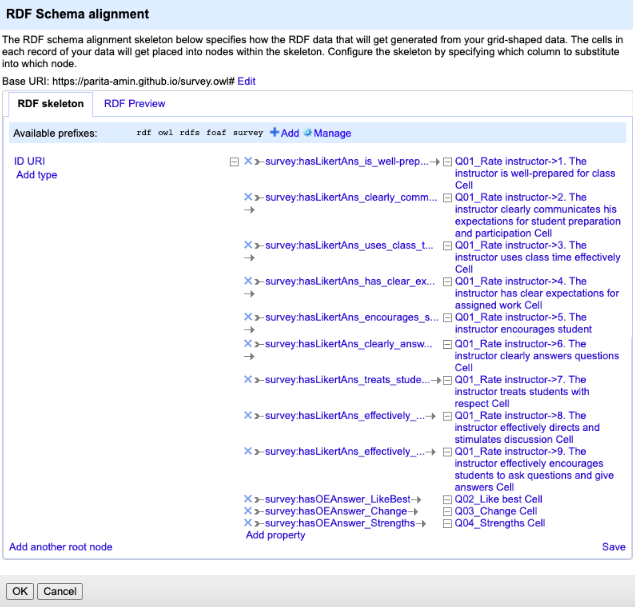
\includegraphics[width=15cm]{images/ch4/survey/survey-rdf-skeleton.png}
    \caption{RDF Skeleton for CSV using Survey Ontology}
    \label{survey-rdf-skeleton}
\end{figure}

\begin{figure}[htp]
    \centering
    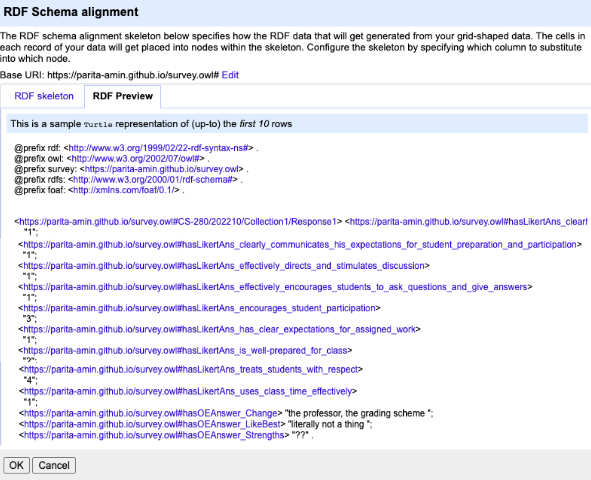
\includegraphics[width=15cm]{images/ch4/survey/survey-rdf-preview.png}
    \caption{RDF Preview for CSV using Survey Ontology}
    \label{survey-rdf-preview}
\end{figure}

\section{Licensing Survey Vocabulary}



\section{Publishing Linked Open Vocabulary for Survey}



\section{Visualization Tools for \ac{owl} Ontology}

The next step is visualization of the built \ac{owl} ontology using various visualization tools. Protégé supports plug-ins for some visualization tools like OntoGraf and \ac{owl}Viz whereas tools like WebVOWL, RelFinder and \ac{owl}GrEd are available for use as web-based tools. This section focuses on the two tools, OntoGraf and WebVOWL, used for the visualization of the survey ontology in this research.

\subsection{OntoGraf}

Falconer~\cite{falconer2010ontograf} introduced OntoGraf as a protégé plug-in for the visualization of the \ac{owl} ontologies. This tool helps the users to represent the ontologies, built using protégé, by repetitively allowing and restricting the desired classes. OntoGraf offers various graph layout options for visualization like Grid Layout\footnote{classes are arranged in a grid alphabetically}, Spring Layout, and Tree Layout\footnote{both horizontal and vertical}. Antoniazzi and Viola~\cite{antoniazz2018rdf} stated that the \say{individuals of a class can be visualized in its tooltip, but this is uncomfortable when dealing with a high number of assertional statements}. The graphs generated using OntoGraf can be exported as image files of various formats such as \ac{png}, \ac{jpeg}, \ac{gif} and as a dot file\footnote{a Microsoft Word Template with the details of default settings}.

Figure~\ref{ontograf} shows the graph generated using OntoGraf for the survey ontology. To start with the graph formation, the classes \say{Thing}, \say{Domain\_entity}, \say{Independent\_entity} and \say{Value} were selected followed by expansion of \say{Independent\_entity} and \say{Value} classes by double-clicking them. This expansion adds all the classes that are connected to the classes. The classes connected includes both the subclasses as well as the ones linked through the object properties. Solid blue lines are used to denote the relationships between the classes and their subclasses whereas dashed lines are used to represent the object properties.

\begin{figure}[htp]
    \centering
    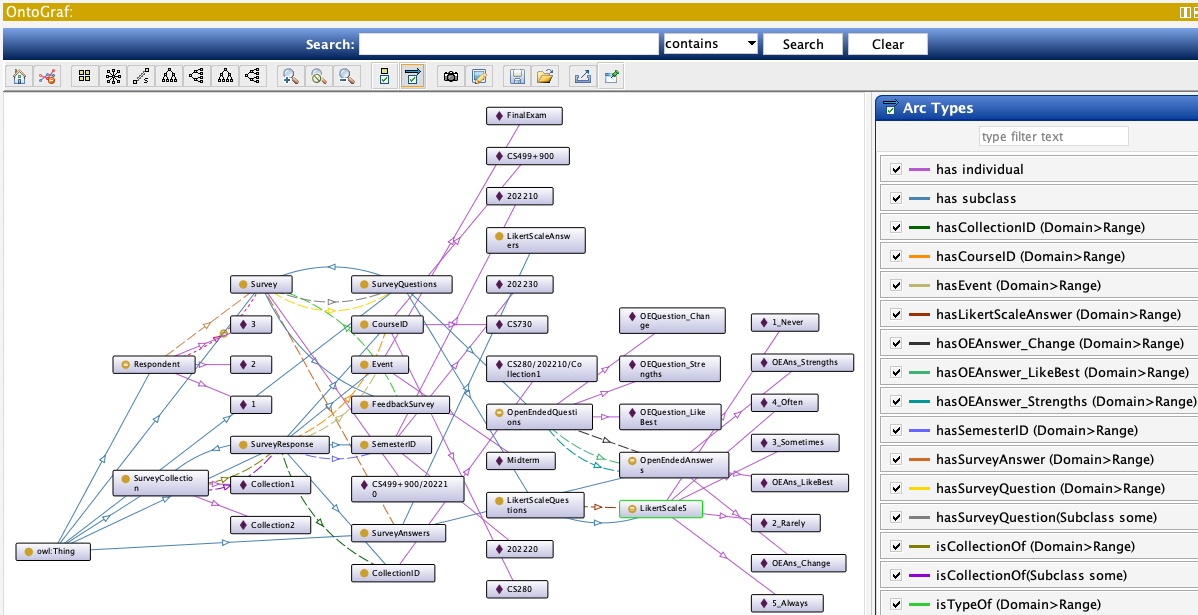
\includegraphics[width=15cm]{images/ch4/survey/ontograf.png}
    \caption{OntoGraf for Survey Ontology}
    \label{ontograf}
\end{figure}

\subsection{WebVOWL}

WebVOWL~\cite{lohmann2014webvowl}, the Web-based \ac{vowl}, one of the variety of forms in which the \ac{vowl} visualization tool is available, represents the \say{ontologies graphically using a force-directed graph layout}~\cite{antoniazz2018rdf}. \ac{vowl} follows some ground rules for the representation of \ac{owl} ontologies which are:

\begin{enumerate}
  
    \item Circles are used to denote classes. Also, different types are assigned different colors. For instance, \ac{owl} classes are denoted using \say{light blue circles}.

    \item Black solid lines are used to represent \ac{owl} object and datatype properties. The object properties use light blue labels where as the datatype properties are labelled in green.
  
    \item The relationships between the classes and their subclasses are represented using dashed lines.

\end{enumerate}

Figure~\ref{webVOWL} shows the graphical representation of the survey ontology using Web\ac{vowl}. The figure focuses on only some of the class-subclass relationships and some of the object properties. The metadata and the statistics of the node (circle) or the edge (line) can be retrieved by clicked on them. The entities (classes) and their relationships (object and datatype properties) can be presented or restricted using filters. The \ac{vowl} graph can be exported as an \ac{svg} image file or a \ac{json} code file.

\begin{figure}[htp]
    \centering
    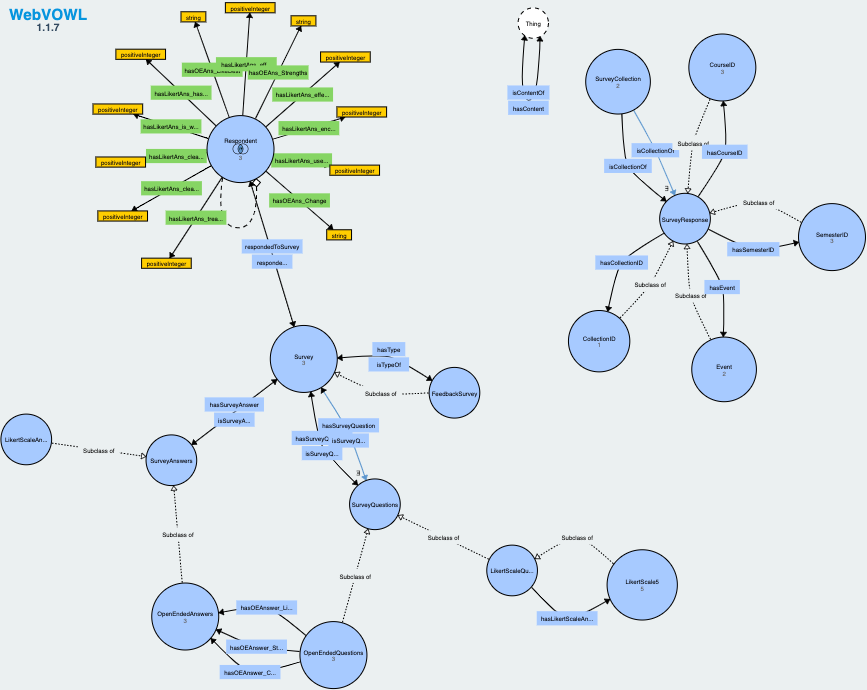
\includegraphics[width=15cm]{images/ch4/survey/webVOWL.png}
    \caption{WebVOWL for Survey Ontology}
    \label{webVOWL}
\end{figure}

\end{doublespace}